\documentclass[journal]{IEEEtran}
\usepackage[caption=false,font=footnotesize]{subfig}
\usepackage{booktabs}
\usepackage{datatool}
\usepackage{listings}
\usepackage{makecell}
\usepackage{tikz}
\usetikzlibrary{positioning}
\usetikzlibrary{trees}
\usetikzlibrary{fit}
\usetikzlibrary{backgrounds}
\usepackage[hyphens]{url}
\usepackage{hyperref}

\lstdefinestyle{lststyle}{
	aboveskip=20pt,
	belowskip=20pt,
	frame=single,
	basicstyle=\tt\scriptsize,
	commentstyle=\color{gray}}

\begin{document}
\DTLloaddb{keys_values}{results/keys-values.csv}

\title{Reproducible Builds for\\ Computational Research Papers}

\author{Paschalis~Bizopoulos and Dimitris~Bizopoulos
\thanks{P. Bizopoulos and D. Bizopoulos are Independent Researchers, Thessaloniki, Greece e-mail: pbizopoulos@protonmail.com, dimitrisbizopoulos@gmail.com}}

\maketitle

\begin{abstract}
	Previous works in research reproducibility provided frameworks for writing reproducible research papers, however without considering the extra work that needs to be done by the author to make his paper reproducible and by the reviewer to verify the paper's reproducibility.
	We propose a simple template for writing computational research papers in \LaTeX\ that are easily verifiable in terms of their reproducibility.
	The template contains a Makefile that allows the verifier to execute the code that reproduces the figures, tables and variables (results) of the paper, which are then used during the \LaTeX\ compilation, to produce a pdf.
	The previous procedure is completed twice and the paper is verified as reproducible, if and only if the pdf files are identical.
	The two builds are needed to enable comparison between different builds of the same source code such that any non-deterministic stochasticity would produce different pdf files, thus making the paper non-reproducible.
	The reproducibility of a paper can be verified either locally on the machine of the verifier or remotely using Virtual Machines (VMs) in the cloud.
	We release an open source template of \textit{reproducible builds} (RBs) and use it to write and verify the reproducibility of this paper.
\end{abstract}

\section{Introduction}
A research paper is considered reproducible when any reviewer is able to reproduce its results, given the data and experimental procedure.
More specifically, computational research reproducibility requires the presence of source code that produces or fetches data from external sources which then transforms into the figures, tables and variables of the paper.
Open sourcing the code and the raw data of a computational research paper increases its reproducibility confidence but it is not enough to verify it.
Using a template for writing and verifying computational research papers will push the direction towards creating reproducible research, thus tackling the `reproducibility crisis' problem.

We propose a template that uses the concept of \textit{reproducible builds} (RBs) to verify the reproducibility of computational research papers written in \LaTeX.
The template consists of a Makefile that allows the verifier to execute the source code that produces the figures, tables, variables (results), and later compile the \LaTeX\ to produce a pdf.
The previous procedure is executed twice and the research paper is verified as reproducible, if and only if the resulting pdf files are identical.
This procedure can be executed either locally in the verifier machine or remotely in Virtual Machines (VMs) in the cloud.

We provide an open source implementation of the template\footnote{\url{https://github.com/pbizopoulos/cookiecutter-reproducible-builds-for-computational-research-papers}} for writing papers with RBs and use it to write this paper\footnote{\url{https://arxiv.org/abs/2005.12660}} and verify its reproducibility\footnote{\url{https://github.com/pbizopoulos/reproducible-builds-for-computational-research-papers}}.
We use Python~\cite{van2007python} for producing the results, however other scientific-oriented programming languages such as R~\cite{ihaka1996r} and Julia~\cite{bezanson2017julia} can be used.

For the rest of the paper we will refer to:
\begin{itemize}
	\item \textit{paper} as a computational research paper,
	\item \textit{results} as the figures, tables and variables that are shown in the paper,
	\item \textit{\LaTeX\ code} as the files containing the main text (\textit{*.tex} files) and bibliography (\textit{*.bib} files) of the research paper,
	\item \textit{results code} as the files containing the scientific-oriented programming language code (\textit{*.py} files) that produces the results and
	\item \textit{code} as both the \textit{\LaTeX\ code} and \textit{results code}.
	\item \textit{author} as the author or authors of the \textit{paper},
	\item \textit{reviewer} as the reviewer of the \textit{paper},
\end{itemize}

\section{Reproducible Builds Template}

\begin{figure}[!t]
	\centering
	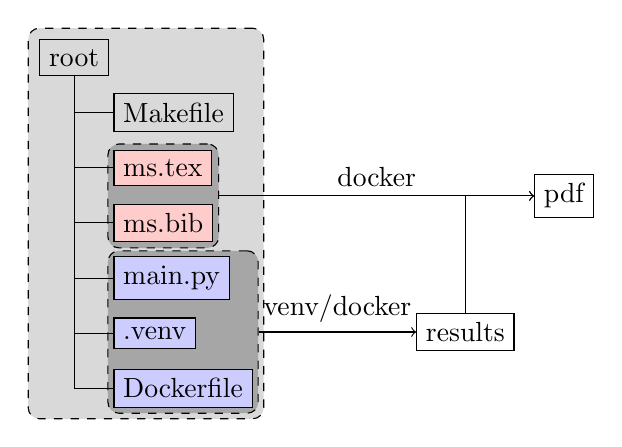
\begin{tikzpicture}[%
			grow via three points={one child at (0.5,-0.7) and two children at (0.5,-0.7) and (0.5,-1.4)},
			edge from parent path={(\tikzparentnode.south) |- (\tikzchildnode.west)}]
			\node[draw](root){root}
			child{node[draw, anchor=west](makefile){Makefile}}
			child{node[draw, anchor=west, fill=red!20](tex){ms.tex}}
			child{node[draw, anchor=west, fill=red!20](bib){ms.bib}}
			child{node[draw, anchor=west, fill=blue!20](py){main.py}}
			child{node[draw, anchor=west, fill=blue!20](venv){.venv}}
			child{node[draw, anchor=west, fill=blue!20](dockerfile){Dockerfile}};
			\begin{scope}[on background layer]
				\node[draw, rounded corners, dashed, fill=gray!30, inner sep=4pt, fit=(root) (dockerfile)]{};
				\node[draw, rounded corners, dashed, fill=gray!70, inner sep=2pt, fit=(py) (dockerfile)](code){};
				\node[draw, rounded corners, dashed, fill=gray!70, inner sep=2pt, fit=(tex) (bib)](paper){};
			\end{scope}
			\node[draw, right=2cm of code, fill=white] (results) {results};
			\path[draw, ->] (code) -- node[above]{venv/docker} (results);
			\node[draw, right=4cm of paper, fill=white] (pdf) {pdf};
			\path[draw, ->] (results) |- (pdf);
			\path[draw, ->] (paper) -- node[above]{docker} (pdf);
	\end{tikzpicture}
	\caption{The RBs template file hierarchy is depicted in the light gray background and the arrows denote the data flow towards generating the pdf.
	Blue indicates a \textit{results code} file, red a \textit{\LaTeX\ code} file and within the dark gray background files that are used for a subsequent step.}
	\label{fig:filehierarchyworkflow}
\end{figure}

The proposed template can be applied on computational research papers written in \LaTeX~\cite{lamport1994latex} and the \textit{results code} can be executed within a Docker container or a virtual environment.
\LaTeX\ is a typesetting system for publishing high quality research papers, and Docker~\cite{merkel2014docker} is a container system that allows portable execution of a codebase between different operating systems/environments and has shown great promise in reproducible research~\cite{boettiger2015introduction}.
The corresponding Dockerfile can be provided by the \textit{author} or generated by tools such as containerit~\cite{nust2019containerit}.

A specific file hierarchy (shown in Fig.~\ref{fig:filehierarchyworkflow}) is used in this paper however this is optional, as the template only needs to know the directories of the main files of the \LaTeX\ and \textit{results code} during its creation by the template.
The template fits in the research writing and reproducibility verificatrion in the following way:
\begin{enumerate}
	\item the \textit{author} writes or edits code in his local repository,
	\item the \textit{author} may verify the reproducibility of the paper locally,
	\item the \textit{author} may push the change to the remote repository, which optionally triggers the remote reproducibility verification:
		\begin{enumerate}
			\item two VMs (builders) execute the \textit{results code},
			\item the results along with the \textit{\LaTeX\ code} are used to compile the pdf files,
			\item the pdf files are sent to another VM (verifier), which verifies the research paper as reproducible if and only if the pdf files are identical.
		\end{enumerate}
	\item the \textit{reviewer} can check the remote reproducibility verifcation or if not available locally verify the reproducibility in his own machine.
\end{enumerate}

Docker usage in RBs provides portability of the environment of the research while the VM provides trust in the procedure (in contrast in executing these local, thus having low credibility in reporting reproducibility).
The reason that two independent builder VMs are needed is to enable comparison between different builds of the same source code and any non-deterministic stochasticity (such as not applying a specific seed to random generators) would produce different pdfs, thus making the verifier VM report the paper as non-reproducible.

Additional constraints could be imposed in the VMs such as disallowing image files in the code and monitoring the network connections of the \textit{code} to help the \textit{reviewer} check whether the results are generated from the \textit{code} and are not fetched from an external source.

Other potential uses of the RBs template include:
\begin{itemize}
	\item Preprint server (such as arXiv) results reproducibility verification.
		The difference with the remote reproducibility verification is the presence of an additional VM that checkouts the \textit{\LaTeX\ code} and generates a pdf which is then compared with the one generated from \textit{code}.
	\item Regression testing and debugging, to ensure that changes to the code do not alter the results.
\end{itemize}

\subsection{Technical implementation}
An open source implementation of the RBs template is available in which the remote reproducibility verification is done using Github Actions.
The builder VMs use different versions of Ubuntu (18.04 and 20.04) and pull a docker image for building \LaTeX\ from DockerHub.
We demonstrate its use by writing and verifying the reproducibility of this paper and its arXiv version.

Regarding research that is computational costly, the template provides a debug flag that verifies the reproducibility of a computationally lighter version of the paper.
This flag also helps in faster iterations during research writing and experimentation.
An example of the debug flag in the field of neural networks is setting the number of epochs and number of training samples to a low value.

Some possible executions that RBs provide are summarized in the following syntax:
\begin{lstlisting}[language=Bash, style=lststyle, caption={Makefile call syntax from the shell.}, captionpos=b]

make [OPTION] [ARGS=--full] [GPU='--gpus all']

OPTIONS
# (or empty OPTION) Generate pdf with results from venv.
ms.pdf
# Verify venv paper reproducibility.
venv-verify
# Generate pdf with results from docker.
docker
# Verify docker paper reproducibility.
docker-verify
# Remove cache, results, venv directories and tex aux files.
clean
# Show help.
help
\end{lstlisting}

The RB template takes advantage of the automatic generation of intermediate files of the `make' program.
The \textit{author} only needs to edit (or use the `touch' program to force) a file from \textit{results code} or \textit{\LaTeX\ code} and the corresponding compilation is automatically triggered.

\section{Discussion}
Previous works in this area such as Hurlin et al.~\cite{hurlin2019reproducibility} propose an `external certification agency' for economic studies.
RBs provide a simple solution for writing and verifying the reproducibility of a computational research paper as a whole, without having to trust a third-party.
Anyone can clone a repository written with RBs and locally verify its reproducibility, in case third party verifications (such as cloud VMs) cannot be trusted.

\section{Conclusion}
Automating research reproducibility verification is becoming more important due to the increasing research output that has been observed in the last few years.
Few works were done on this area, mostly proposing trust on an external third party.
RBs help in writing and verifying reproducible research using the tools that most of the researchers already use (\LaTeX, Docker).

\section{APPENDIX - Improving Computational Research Reproducibility}
This appendix provides suggestions for improving the reproducibility of computational research papers written in \LaTeX\ with Python as the \textit{results code} programming language.
For demonstration purposes we train and test a simple neural network on the MNIST~\cite{lecun2010mnist} dataset with PyTorch~\cite{paszke2019pytorch}.

A common culprit against reproducibility in \LaTeX\ is the time-date metadata of pdf output.
These can be disabled using the following into the \textit{\LaTeX\ code} after the preamble or as extra arguments during \LaTeX\ compilation (as done in the RB Makefile):
\begin{lstlisting}[language=TeX, style=lststyle, caption={\LaTeX\ pdf reproducibility commands.}, captionpos=b]
\pdfinfoomitdate=1
\pdfsuppressptexinfo=-1
\pdftrailerid{}
\end{lstlisting}

A useful \LaTeX\ package for automatically embedding code results variables in \textit{\LaTeX\ code} is \textit{datatool} with the following example use:
\begin{lstlisting}[language=TeX, style=lststyle, caption={\LaTeX\ datatool example of loading a file that contains pairs of keys and values (keys\_values.csv) generated by a \textit{results code} and getting the value of a key named lr.}, captionpos=b]
\DTLloaddb{keys_values}{keys_values.csv}
\DTLfetch{keys_values}{key}{lr}{value}
\end{lstlisting}

For example the values of the following variables are not referred in the main \textit{.tex} file but they are read by an intermediate \textit{.tex} file created by the \textit{results code}:
\begin{itemize}
	\item the learning rate is $\DTLfetch{keys_values}{key}{lr}{value}$,
	\item the batch size is $\DTLfetch{keys_values}{key}{batch_size}{value}$ and
	\item the validation accuracy of the best model is $\DTLfetch{keys_values}{key}{validation_accuracy_best}{value}\%$.
\end{itemize}

Regarding the \textit{results code} for Python, random seeds need to be set to a specific value such as:
\begin{lstlisting}[language=python, style=lststyle, caption={Python reproducibility commands for some popular libraries.}, captionpos=b]
# for build-in random module
random.seed(0)
# for numpy
np.random.seed(0)
# for pytorch
torch.backends.cudnn.benchmark = False
torch.backends.cudnn.deterministic = True
torch.cuda.manual_seed_all(0)
torch.manual_seed(0)
# for Tensorflow
tf.random.set_seed(0)
\end{lstlisting}

Using the random seeds and \textit{datatool} we could have deterministic stochasticity that reproduces figures, tables and variables.
For example Fig.~\ref{fig:image} depicts the train and validation loss:
\begin{figure}[h]
	\includegraphics[width=\linewidth]{results/image.pdf}
	\caption{Image example created from \textit{results code}.}
	\label{fig:image}
\end{figure}

Another useful results function for Python is \textit{pandas.DataFrame.to\_latex} which automatically converts a dataframe table to a \LaTeX\ table (as shown in Table~\ref{table:table}.

\begin{lstlisting}[language=python, style=lststyle, caption={Convert Pandas DataFrame to \LaTeX\ table.}, captionpos=b]
num_columns = 11
table = np.random.random((7, num_columns))
df = pd.DataFrame(table)
df.to_latex('table.tex', float_format="%.2f")
\end{lstlisting}

\begin{table}[h]
	\centering
	\caption{Table example created from \textit{results code}.}
	\label{table:table}
	\setlength\tabcolsep{4.2pt}
	\input{results/table.tex}
\end{table}

\bibliographystyle{IEEEtran}
\bibliography{ms}

\end{document}
